
\chapter{Discussion}    
\label{Ch:discussion}

Recruitment and function of the Rvs complex in has been explored in this work, as well as several models for how membrane scission could be effected in yeast endocytosis. 
I propose that Rvs localizes by interactions of the BAR domains of the Rvs complex with invaginated membranes, and that the SH3 domain is required for efficient recruitment of Rvs to sites. Arrival of Rvs on membrane tubes scaffolds the membrane tube and prevents membrane scission, in a manner that depends on recruitment of a critical number of Rvs molecules, till actin forces rupture the membrane, causing vesicle scission, and releasing Rvs molecules. Here I discuss the main findings of this thesis in support of these propositions.



\section{Recruitment of Rvs to endocytic sites}
Rvs is relatively short-lived protein at endocytic sites, recruited only once membrane tubes once they are formed (Picco et al. 2015; Kukulski et al. 2012; Kaksonen, Toret, and Drubin 2005). FCS measurements have shown that the cytoplasmic content of Rvs167 and Rvs161 is quite high compared to other endocytic proteins (Boeke et al. 2014). Many endocytic proteins like Las17, Vrp1, type1 myosins, are measured at 80-240nM, while cytoplasmic intensity of Rvs161 and 167 is 721nM and 354nM respectively. In spite of this, relatively few numbers of Rvs are recruited to endocytic sites, suggesting that cytoplasmic concentration alone may not determine recruitment. Comparison between FCS measurements of cytoplasmic concentration for different endocytic proteins, and their recruitment to the endocytic sites indicates low correlation between the two, perhaps unsurprisingly, requiring that other directed mechanisms recruit proteins in a timed and efficient manner. In the case of Rvs, both timing and efficiency appear crucial to its function, the question is what confers both. 


%\subsection{Timing of localization and efficiency of recruitment}

\subsection{The BAR domain senses membrane curvature}
The curved structure of the BAR dimer has suggested that Rvs is recruited by its preference for some membrane shapes over others, supported by its arrival at curved membrane tubes. In the absence of membrane curvature, in sla2Δ cells, the BAR domain alone does not localize to cortical patches (Fig.3.3D). This demonstrates for the first time that the BAR domain does indeed sense and requires membrane curvature to localize to cortical patches. Work on BAR domains have proposed that electrostatic interactions between positive charges at the concave surface and tips of the BAR domain structure and negatively charged lipids mediate membrane binding. Mutations in these lipid-binding surfaces would clarify the interaction with underlying lipids, and test if Rvs relies on similar interactions.



\subsection{BAR domain times recruitment of Rvs} 

In BAR cells, Rvs167 is able to localize to endocytic sites, and has a similar lifetime in WT cells (Fig.3.3, Fig.3.4). In Fig.3.4 B,D we see that while in WT, Rvs167 arrives about 4 seconds after the arrival of Abp1, in BAR cells it arrives only 6 seconds after Abp1 arrives. There is a time delay between Abp1 and Rvs167 recruitment in BAR cells, confirmed by the TIRF measurement in 3.4D. 

	\vspace{5mm}
The delay in recruitment could occur because the membrane has not acquired the required invagination lengths or because the loss of the SH3 domain has delayed recruitment. That the delay comes from the absence of a particular invagination length is supported by the fact that Sla1 moves inwards at a slower rate in BAR cells. It takes longer for the membrane in BAR cells to reach the same length as WT. Rvs167 arrives in BAR cells when Sla1 has moved inwards 25-30nm (dashed red lines in Fig.3.4A), which is also the distance Sla1 has moved when Rvs167 arrives in WT. To be noted is that Sla1 is not directly at the plasma membrane, and the centroid of Sla1 sits about 20nm higher on the plasma membrane than Sla2(Picco et al. 2015). Therefore, a 25-30nm distance of Sla1 would correspond to 45-50nm of membrane invagination, by which point the membrane is already tubular (Picco et al. 2015; Kukulski et al. 2012), consistent with Rvs arrival at invaginated tubes. This suggests Rvs recruitment is timed to specific membrane invagination length, and that this timing is provided by the BAR domain. 


\subsection{The SH3 domain makes Rvs recruitment efficient} 
As seen in Fig.3.4C, Rvs167 in BAR cells accumulates to about half the WT number, even though the same cytoplasmic concentration is measured (see methods). This indicates that the SH3 domain increases the efficiency of recruitment of Rvs. Either SH3 domains help recruitment to endocytic sites, or it stabilizes interaction with sites. It is also possible that SH3 domains stabilize dimers of the Rvs complex. Since the cytoplasmic signal of Rvs167 is the same in both WT and BAR cells, and Rvs167 and Rvs161 have been shown to exist as dimers in the cytoplasm (Boeke et al. 2014), it is unlikely that loss of the SH3 domain destabilizes the Rvs complex. In sla2Δ cells, full-length Rvs can assemble on the membrane (Fig.3.3D-F). Since there is no BAR-membrane interaction in sla2Δ cells, this supports a role for the SH3 domain in increasing recruitment of Rvs by clustering protein molecules. 


\subsection{The SH3 domain can assemble and disassemble Rvs molecules independent of the BAR domain and actin interactions} 
As mentioned above, in sla2Δ cells, full-length Rvs is able to localize to cortical patches without the curvature-dependent interaction of the BAR domain (Fig3.3D-F). The independent ability of the SH3 domain to localize and disassemble protein is unexpected. This indicates that the SH3 domain is able to mediate recruitment of an Rvs patch, and then disassemble this patch. 

	\vspace{5mm}
In sla2Δ cells treated with LatA (Fig.3.3G-H), actin-based membrane curvature, as well as actin-binding proteins are removed from the plasma membrane. Full-length Rvs167 in these cells show transient localizations at the plasma membrane (Fig.2A). In BAR + sla2Δ cells with LatA treatment, this localization is lost, suggesting that the former is dependent an SH3 domain interaction, and that this is independent of both actin and membrane curvature. 

Abp1 is an activator of the Arp2/3 complex 

\subsection{SH3 domain times affects actin dynamics}
In WT cells, the Abp1 and Rvs167 fluorescent intensity reach maxima concomitantly, and the consequent decay of both also coincide. That this occurs at the same time indicates that upon vesicle scission, the actin network is immediately disassembled. Membrane scission essentially occurs around the intensity peak of the two proteins. This coincident peak is lost in BAR cells. Rvs in these cells peaks several seconds after Abp1 intensity starts to drop, and the decay of Abp1 is prolonged, taking nearly double the time as in WT. As we see in Fig.3.4C, the number of Abp1 molecules recruited is decreased to about two thirds the WT number. Although it is not clear what the decoupling of Abp1 and Rvs peaks mean, the changes in Abp1 dynamics suggests a strong disruption of the actin network. SH3 domains are known to interact with components of the actin network, but study of other components of the actin machinery is required to understand how exactly loss of the SH3 has changed the progression of endocytosis.  

\subsection{What does the SH3 domain interact with?}
SH3 interaction with an endocytic binding partner could help recruit Rvs to sites. Many such interaction partners have been proposed. Abp1 interaction with the Rvs167 SH3 domain has been shown (Lila and Drubin 1997; Colwill et al. 1999), as has one with WASP protein Las17 (Liu et al. 2009; Madania et al. 1999), yeast Calmodulin Cmd1 (Myers et al. 2016), type I myosins (Geli et al. 2000), and Vrp1 (Lila and Drubin 1997). These proteins are currently being studied as potential targets of the Rvs167 SH3 domain. All of these suggested binding partners localize to the base of the invagination (Yidi Sun 2006; Picco et al. 2015), and do not follow the membrane into the cytoplasm. If one of these is the SH3 interaction partner, SH3 domains interact with the endocytic network at the base of the invagination. Centroid tracking however, suggests that Rvs is accumulated all over the membrane tube without bias towards the base of the invagination. If Rvs was recruited to the base and pulled up as the invagination grows, the centroid would move continuously upwards rather than remain relatively non-motile before the jump at scission time. It is possible that the SH3 initially helps cluster near the base, and as the membrane invaginations grow longer, BAR-membrane interactions dominate. 




%\subsection{Arrangement of Rvs}
	\vspace{5mm}
It is unclear how Rvs is arranged on the membrane tube. Although solved structures of BAR domains show high structural similarity in spite of low sequence similarity, no structure for the Rvs complex exits. The fact that this is a hetero- rather than homodimer suggests that the structure does not necessarily resemble that of Amphiphysin or Endophilin homodimers, and a high-resolution structure will be necessary to clarify the interaction and arrangement of Rvs on endocytic tubes

\subsection{Total number of Rvs recruited is independent of ploidy}
When ploidy is doubled from haploids to diploids, we could expect that double the protein amount is expressed and recruited, but it does not appear so. The amount of Rvs recruited in WT haploid (1xh) and diploids (2xd) remain about the same, and cytoplasmic signal is similar (Fig.4.1). This is not a very robust estimate for cellular expression, and needs to be verified by quantitative western blots. However, the invariance between accumulated protein in haploids and diploids shows that Rvs recruitment is not determined by the number of alleles of Rvs. Haploid and diploid cells appear to tune the amount of Rvs recruitment to get a specific amount to endocytic sites.

	\begin{figure}[H]
	\centering
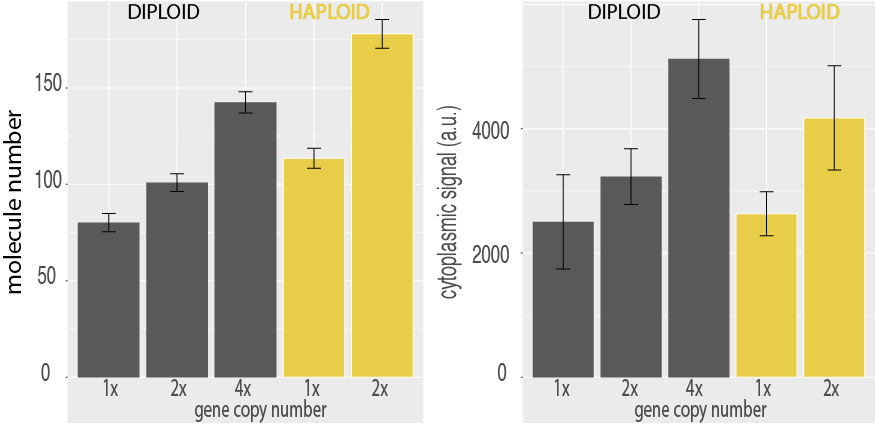
\includegraphics[width=13cm,height=15cm,keepaspectratio]{figures/discussion/number_comp2}
	\caption[Synaptojanin-like proteins in yeast]
	{A. Maximum molecule number of Rvs167-GFP recruited with S.E.M in haploid and diploid cells with different gene copies of Rvs. 
	B. Cytoplasmic signal of Rvs167-GFP with standard deviation in haploid and diploid cells with different gene copies of Rvs. 
	\label{concentration}}
	\end{figure}
%	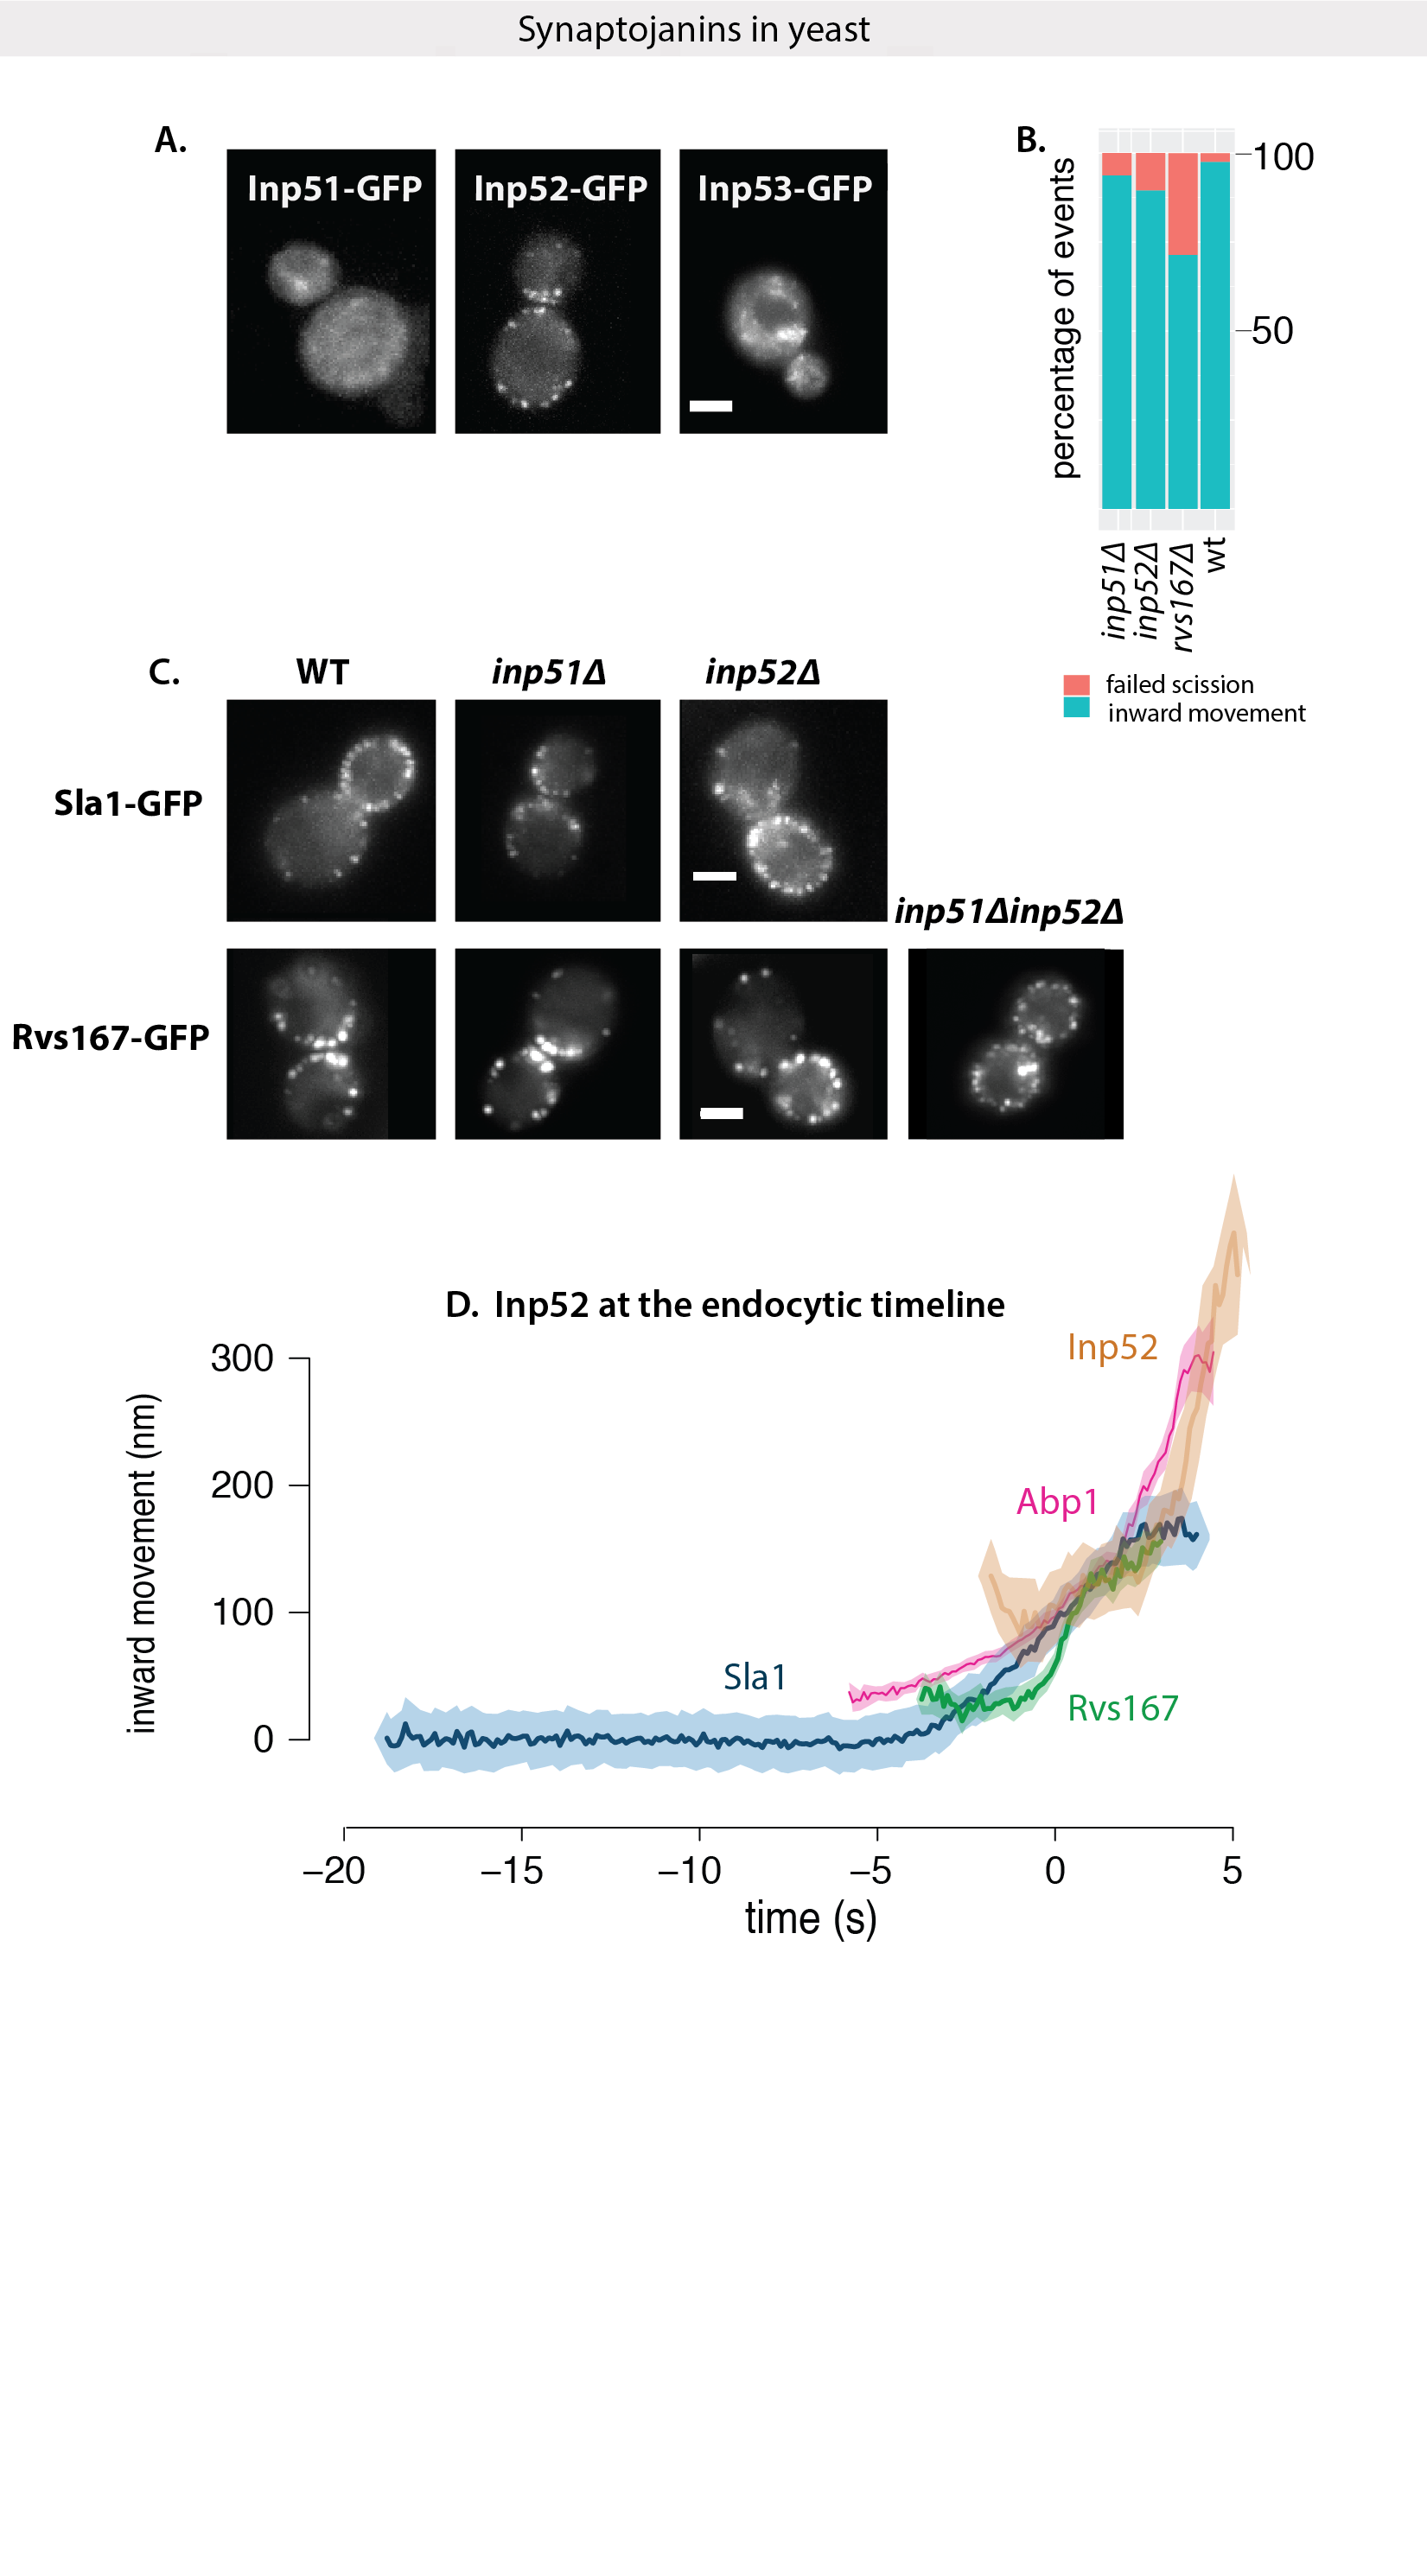
\includegraphics[width=19cm,height=19cm,keepaspectratio]{figures/results_final/inp}

\subsection{Rvs recruitment rate increases with increasing gene copies}
In diploids, the genome that contains four copies of Rvs (4xd) could be expected to express and recruit twice the amount of Rvs as one that contains two copies (2xd). However, cytoplasmic signal increases by 1.6x and recruitment to endocytic sites increases only by 1.4x. Doubling the gene copies appears not to double protein expression or recruitment in the case of Rvs. Similarly, duplicating Rvs genes in haploids results in an increase in number of molecules recruited, but not in doubling (1xh, 2xh). Although the rate of adding Rvs is different in haploids and diploids, in both cases, it increases by gene copy number. 

	\begin{figure}[H]
	\centering
	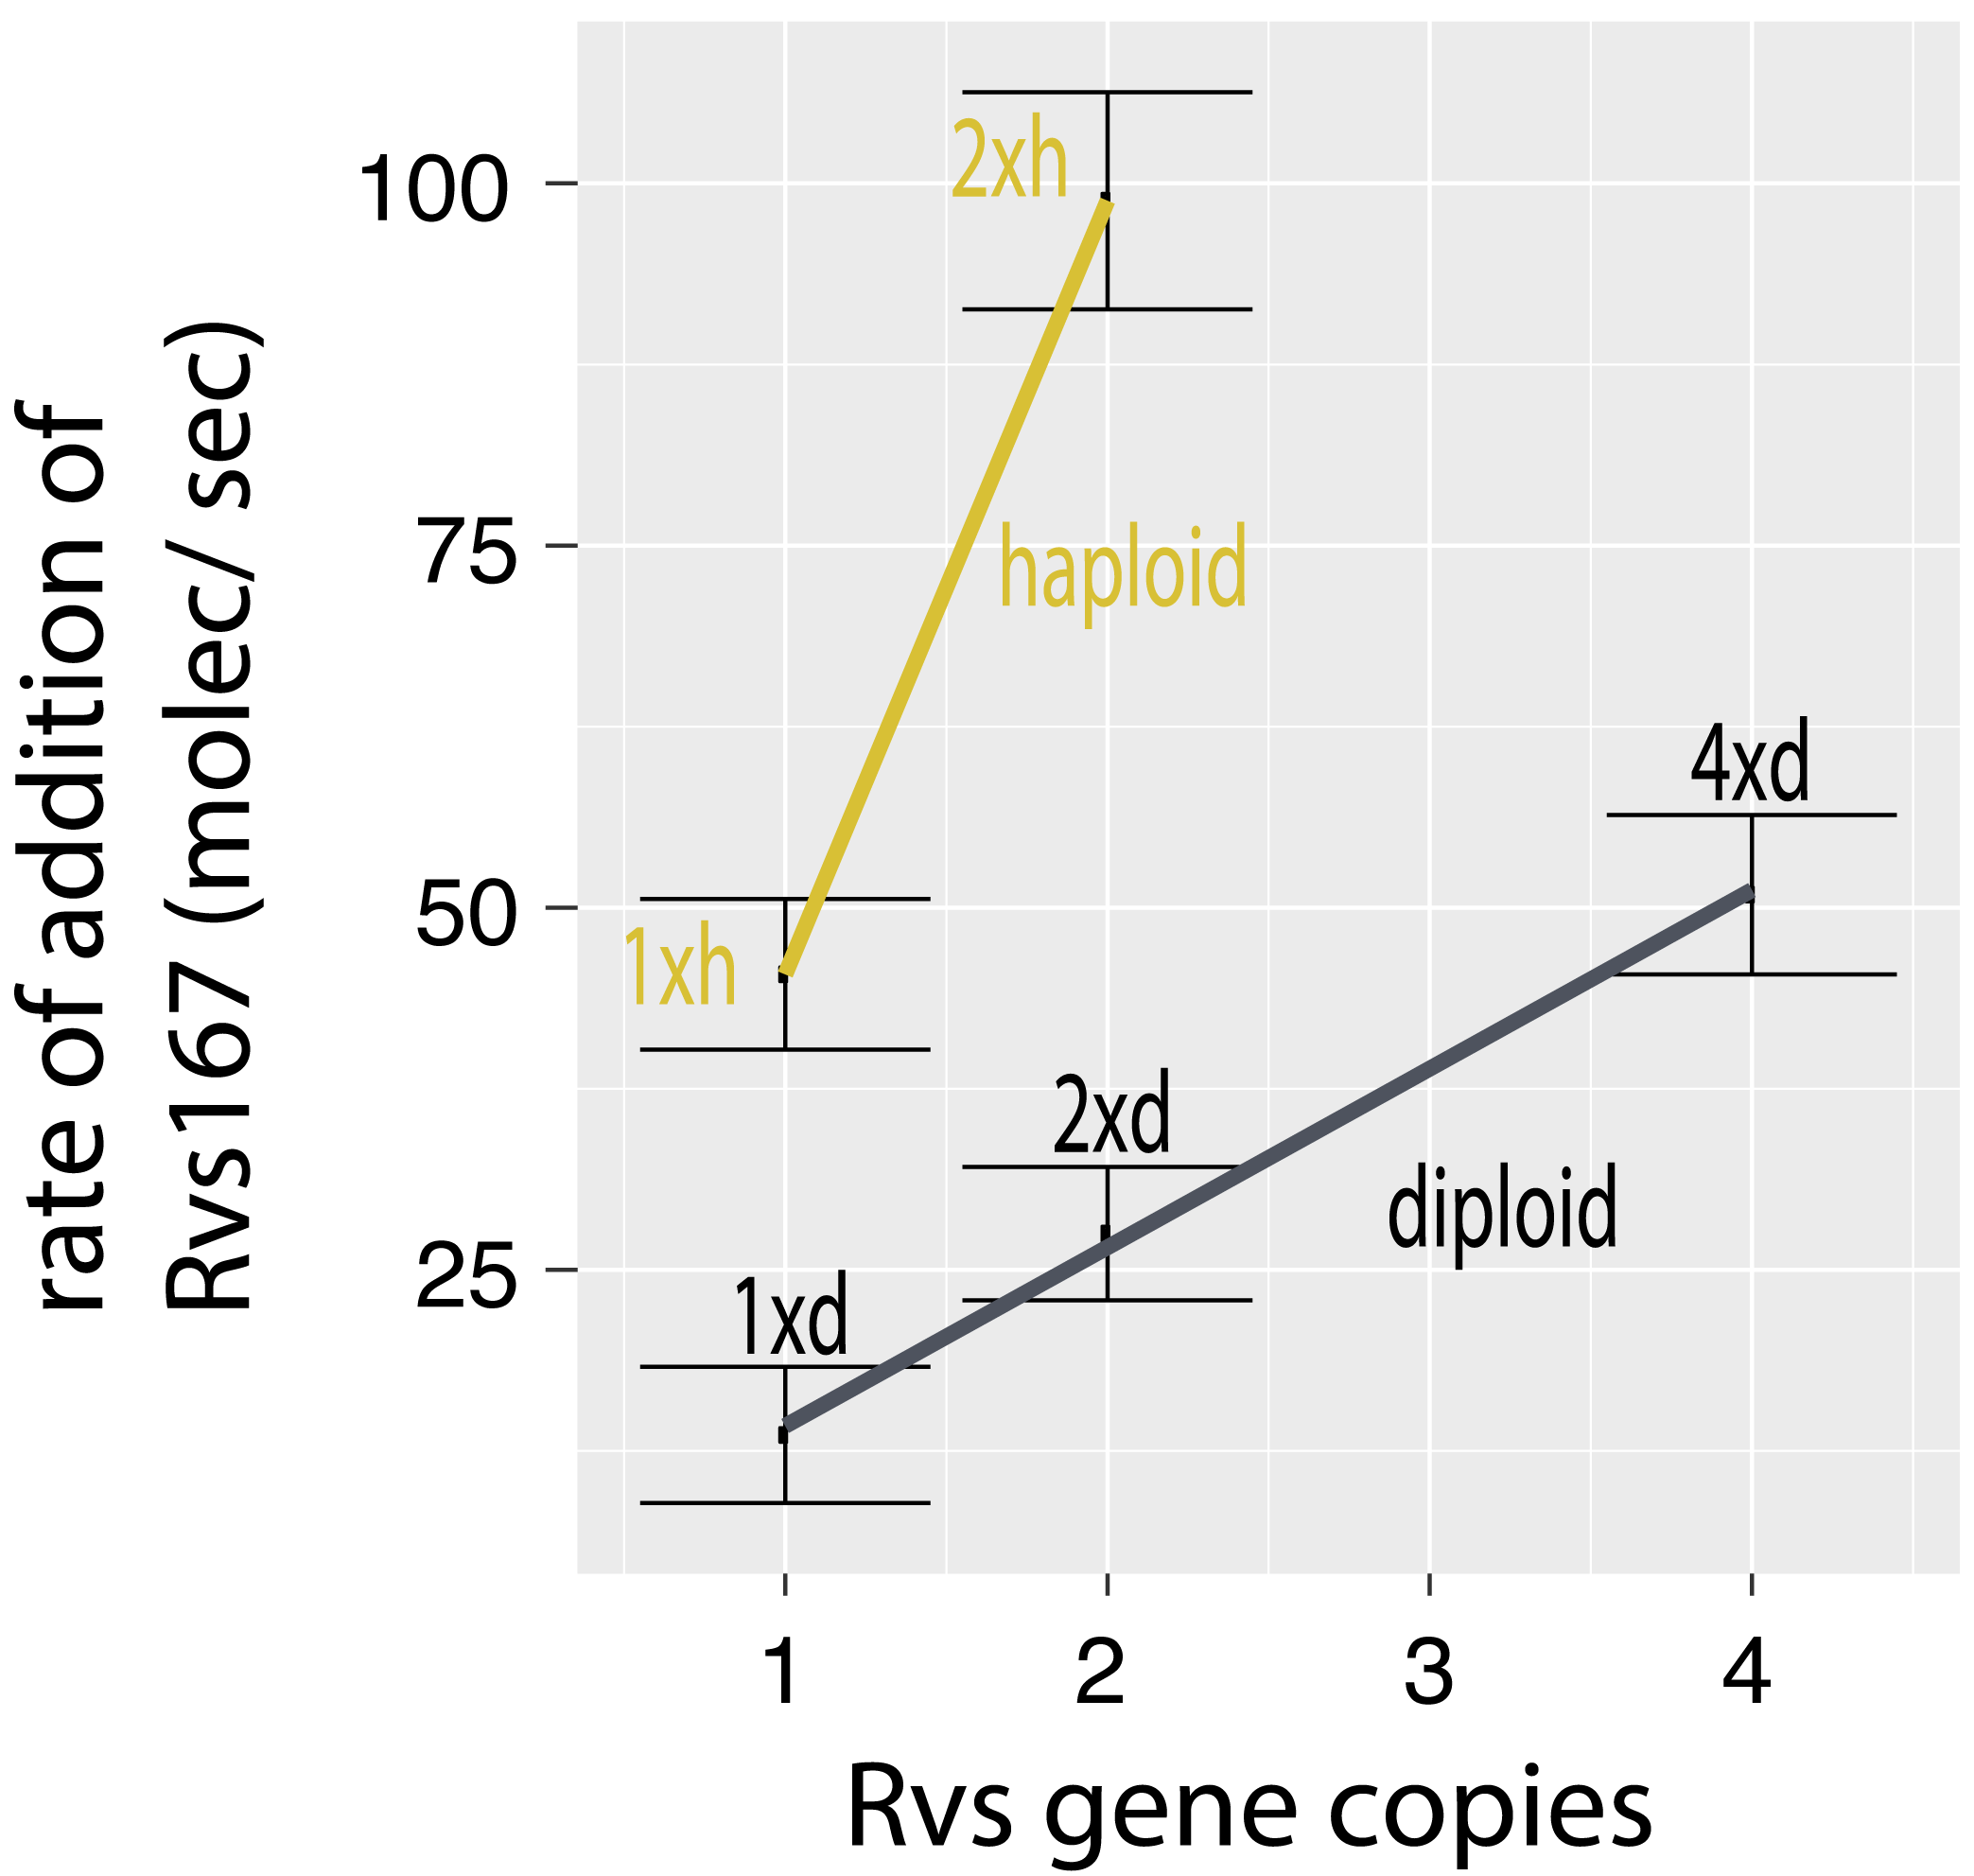
\includegraphics[width=8cm,height=8cm,keepaspectratio]{figures/discussion/recruit_rate_final}
	\caption[Synaptojanin-like proteins in yeast]
{Rate of Rvs molecules added to endocytic sites before scission vs gene copy number in haploids and diploids. SEM of the molecule numbers recruited, and linear fit through the data is shown.
	\label{recruit_rate}}
\end{figure}

	\vspace{5mm}
The rate of Rvs recruitment is slower in WT diploid compared to WT haploid (2xd vs 1xh, Fig.4.2). Diploid cells do not double in volume compared to haploids: under normal growth conditions, the volume of the diploid cell is around 1.57x that of the haploid cell, and the average cell surface area increases to  about 1.4x (Weiss, Kukora, and Adams 1975). It is possible that the delay in recruitment is arises from the fact that protein expression remains the same in both. There is a larger surface area and volume, and more endocytic events in diploids. Recruitment could be delayed in diploids because Rvs is recruited from similarly concentrated cytoplasmic pool to more sites, decreasing the local concentration.

	\vspace{5mm}
Cytoplasmic protein concentration is increased when gene copies are increased, and recruitment to endocytic sites is increased by the increase in cytoplasmic concentration. Although this data needs to be confirmed by quantitative western blots for protein expression, it suggests that how much Rvs is recruited scales with available concentration of protein. 



\section{Arrangement of Rvs}
No solved structure for the Rvs complex exits. That Rvs is a hetero- rather than homodimer suggests that the structure need not resemble that of Amphiphysin or Endophilin homodimers, and a high-resolution detail will be necessary to clarify the interaction and arrangement of Rvs on endocytic tubes. It is therefore unclear how Rvs is arranged, although there are some indications from the experiments in this work of the interaction with the membrane.


\subsection{Rvs does not form a tight scaffold on membrane tubes}
In-vitro helices of BAR domains have suggested that Rvs might form a similar helical scaffold. Correlating CLEM and centroid movements has proposed that an Rvs scaffold covers the entire membrane tube up to the base of the future vesicle (Picco et al. 2015). 

	\vspace{5mm}
In diploid Rvs strains, more Rvs can be recruited, at a much faster rate than in WT cells (Fig.3.9 B-C, Fig.4.2). Disassembly dynamics of 4xd, however, is the same as in 2xd (Fig.3.9C, Fig.4.3). The sharp decay of fluorescent intensity of WT Rvs (1xh in haploids, 2xd in diploids) indicates that all of the protein is suddenly released, consistent with a BAR scaffold that breaks upon vesicle scission, releasing all the membrane-bound protein at once. A similar decay in the 4xd strain suggests that all the Rvs here is also bound to the membrane. Since the membrane is able to accommodate 1.4x the amount of BAR protein as the WT, it would suggest that at lower protein amounts, a tight helix that covers the entire tube is not likely. Adding molecules to such a tube would result in a change in Rvs assembly and disassembly dynamics. Further, additional molecules would have to be added at the top or base of a tight scaffold. At the top, the radius of curvature is decreased compared to the tube since this is the rounded vesicle region. At the base, the plasma membrane is flat, and the Rvs BAR domain is similarly unlikely to favour interactions here. Otherwise the scaffold would have to be disrupted to add new molecules, which would likely slow down recruitment rate rather than speed it up. Molecules could also be added concentric to a pre-existing scaffold. The concave surface of Rvs is known thus far to interact with lipids, and multiple layers of BAR domains on the membrane tube would probably not show the sudden disassembly seen here.  

	\vspace{5mm}
That the membrane surface area does not change in the 4xd compared to 2xd is assumed from the identical movement of Sla1 in both cases (Fig.3.9A). It is possible that a wider tube is formed, which would increase the membrane surface area for BAR binding. This would, however, require the BAR domains to interact with a lower radius of curvature than in WT. This seems unlikely, and in the absence of any indication otherwise, I assume that the membrane tubes in all diploid and haploid cases have the same width.

\subsection{A limit for how much Rvs can be recruited to the membrane}
In the case of Rvs duplication in haploids (2xh), a change in disassembly dynamics is seen (Fig.3.8B, Fig.4.3). In 2xh, the maximum number of molecules recruited is 178 +/- 7.5 compared to WT (1x RVSh) 113.505 +/- 5.2. Nearly 1.6x the WT amount of protein is recruited to membrane tubes. The Rvs167 centroid in 2xh shows a delay in disassembly, suggesting that the excess protein is not directly on the membrane. The excess Rvs either interacts with the actin network via the SH3 domain, or interacts with other Rvs dimers. By a similar argument as 4.2.1 above, I do not expect that multiple layers of BAR domains are formed, and that the excess protein is recruited by the interaction of the SH3 domain.   

	\vspace{5mm}
Whatever the arrangement of the Rvs complex on the membrane, disassembly dynamics is changed in the case of 2xh, compared to all the other haploid and diploid strains. Since the number of Rvs molecules is highest in this strain, this suggests that there is a limit to how much Rvs can assemble on the tube without altering interaction with the endocytic network. 


\begin{figure}[H]
	\centering
	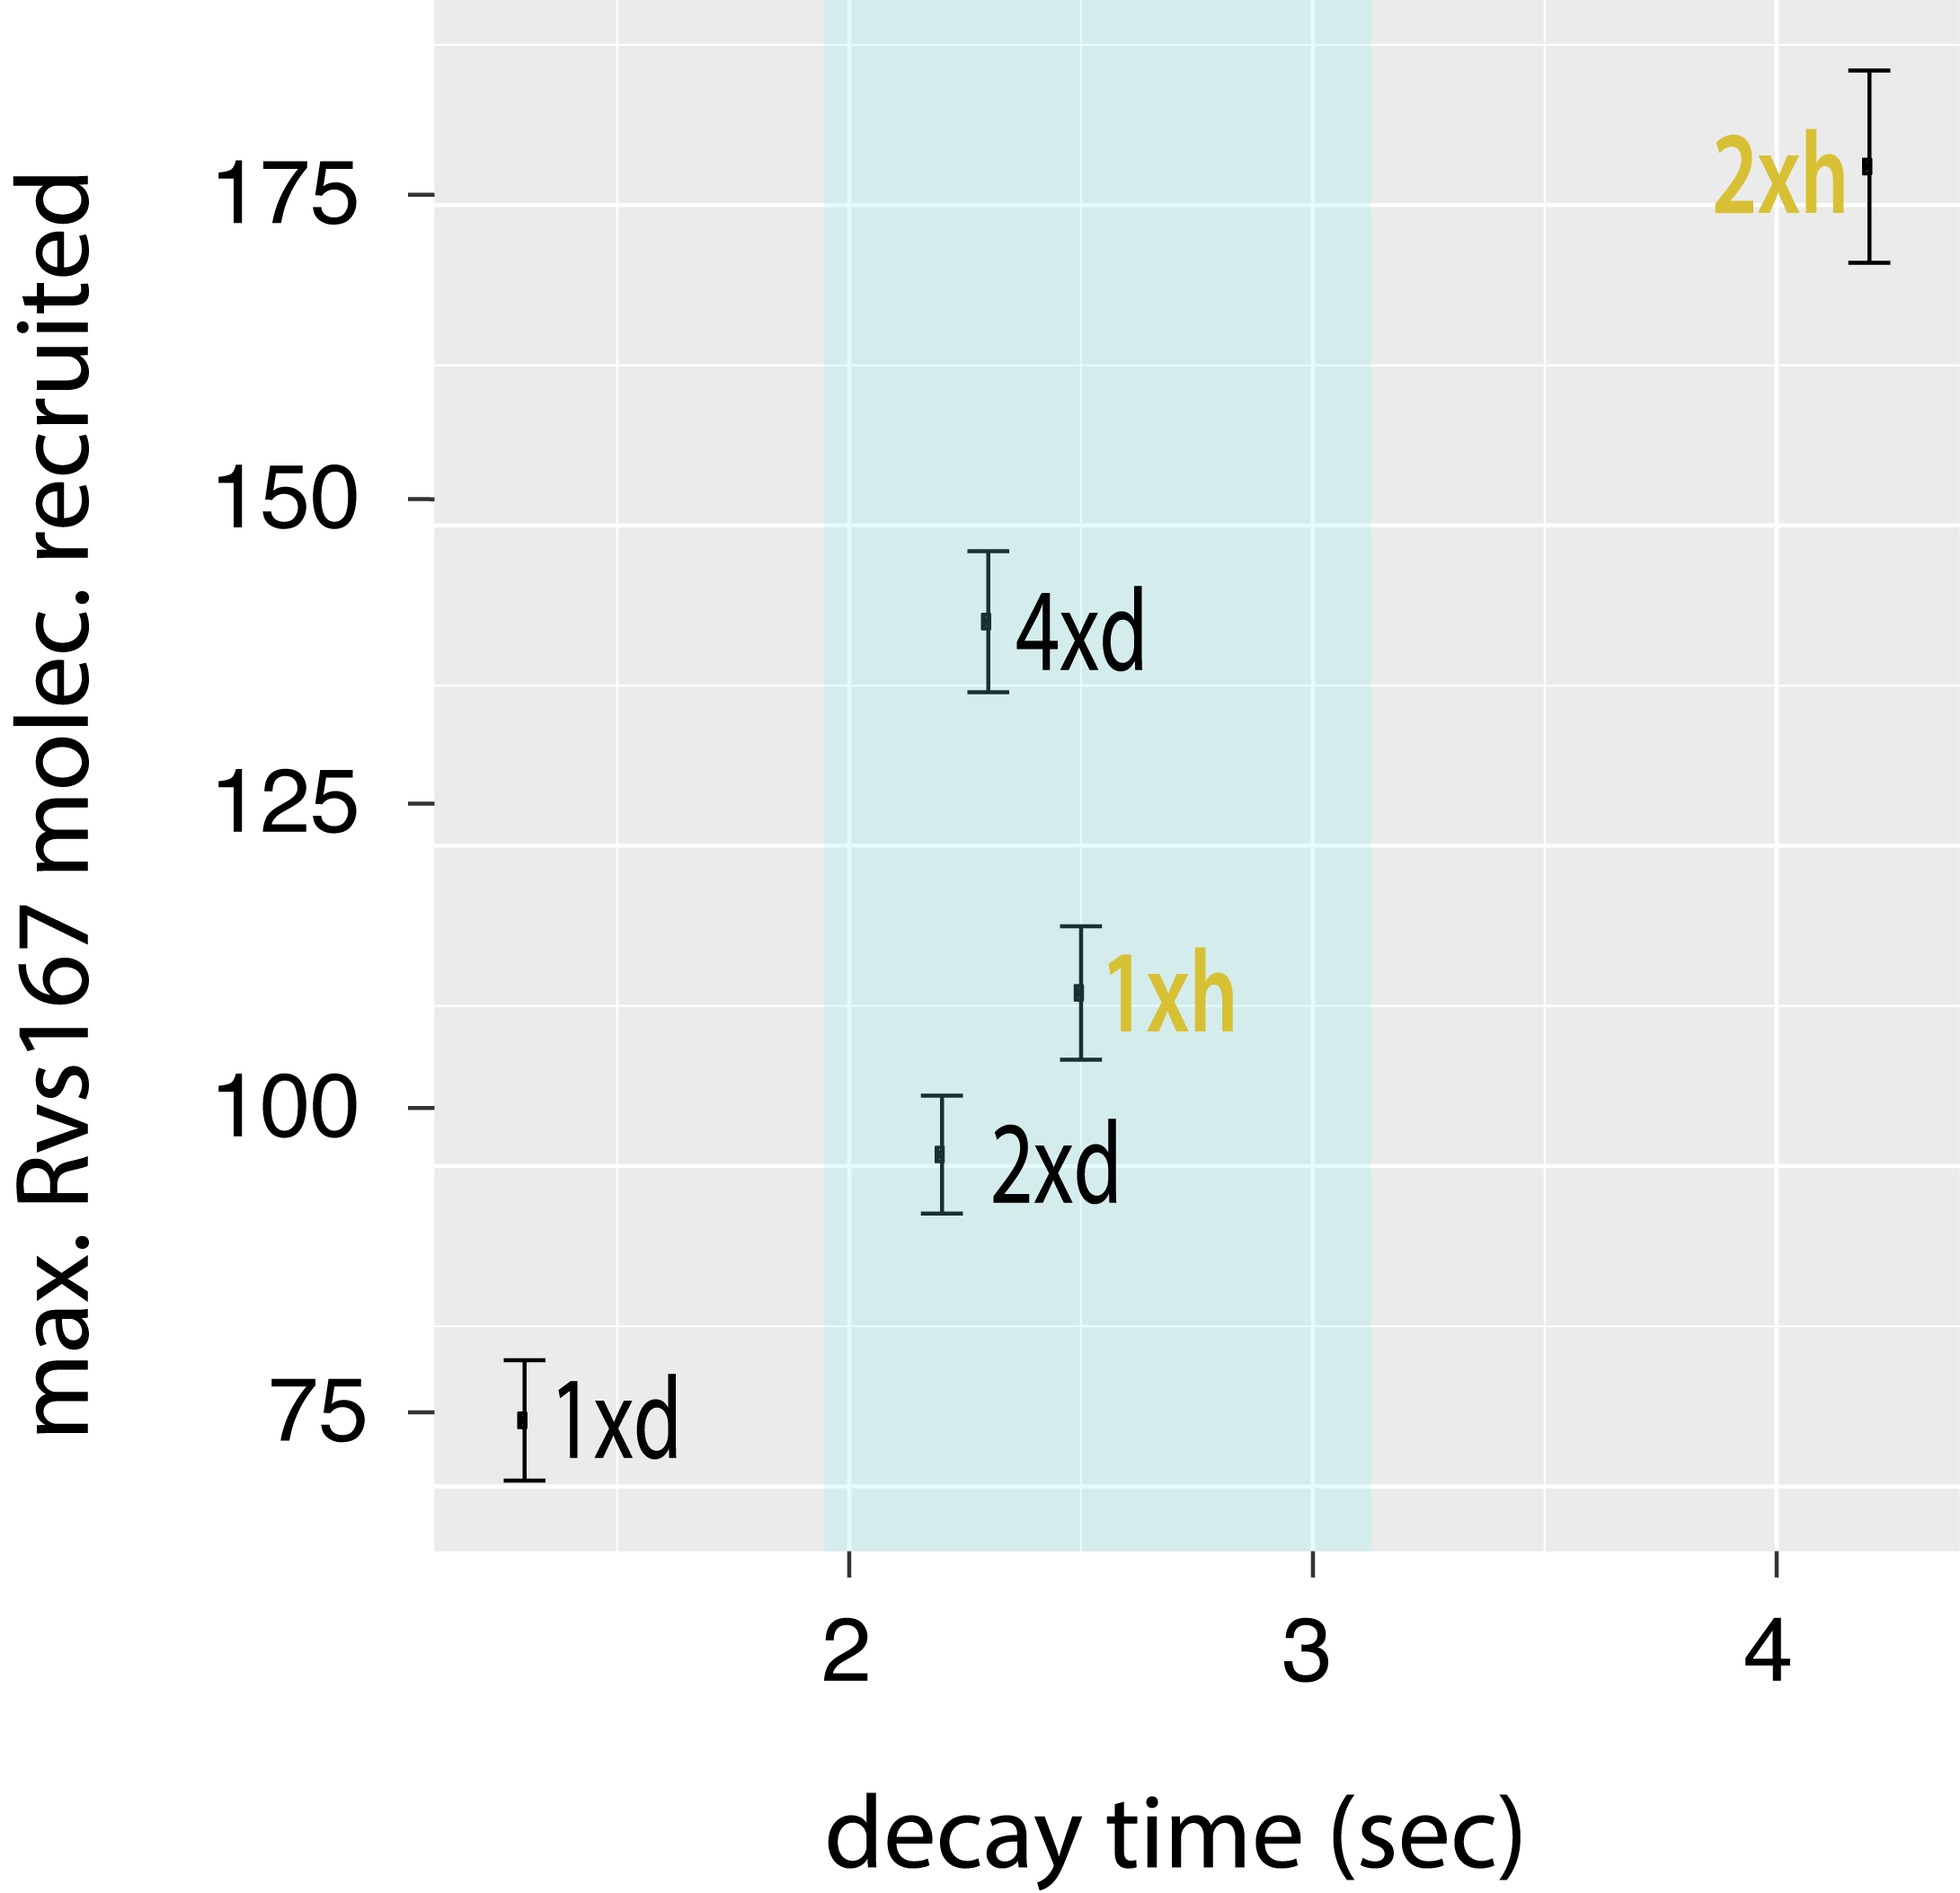
\includegraphics[width=12cm,height=12cm,keepaspectratio]{figures/discussion/decay_final}
	\caption[Synaptojanin-like proteins in yeast]
	{Time from peak of Rvs fluorescent intensity to minimum intensity, against maximum molecule numbers recruited. Coloured region highlights similar disassembly time for increasing amounts of molecules recruited.    
		\label{decay}}
\end{figure}

\subparagraph{Conclusions for Rvs localization }
All of this data supports that Rvs recruitment rate and total numbers is determined by concentration of protein in the cell. The maximum number of molecules can interact with the membrane is limited by the membrane surface area of the invagination tube. Although more can be recruited, Rvs over a certain threshold interacts in a different way with endocytic sites, likely via the SH3 domain. Timing of recruitment to sites is by curvature-recognition via the BAR domain, while efficiency of recruitment and actin interaction is established via the SH3 domain. 


\section{What causes membrane scission?}


\subsection{Dynamin does not not drive scission}
Some studies have suggested that dynamin-like Vps1 localizes to endoytic sites, and affects the scission mechanism: Nannapaneni et al(Nannapaneni et al. 2010)., find that the lifetimes of Las17, Sla1, Abp1 increase in the absence of Vps1. Rooij et al (Rooij et al. 2010)., find that Rvs167 lifetimes increase, and are recruited in fewer patches to the cell cortex. On the other hand, vps1Δ did not increase the scission failure rate of rvs167Δ in other studies (Kishimoto et al. 2011), and did not co-localize with endocytic proteins (Goud Gadila et al. 2017). If Vps1 was to affect scission, the number of failed scission events should increase in vps1Δ cells, but I do not find so, confirming other studies (Kishimoto et al. 2011). Vp1 tagged with super-folded GFP and imaged in TIRF does not form cortical patches that co-localize with Abp1-mCherry (data from Andrea Picco, not shown). GFP-tagging could affect the recruitment of Vps1 to endocytic sites while maintaining its role in other cellular processes like vesicular trafficking. Membrane movement and scission dynamics are however, unchanged in the absence of Vps1. If loss of Vps1 prevented or delayed scission, the membrane would continue to invaginate longer than WT lengths, and Sla1 movements of over 140nm would be measured. Rvs centroid movement would likely also be affected: a bigger jump inwards could indicate that that a longer membrane has been cut. That there are no changes in the behaviour of coat and scission markers indicates that if Vps1 is recruited to sites, it is not necessary for Rvs localization or function, and is not necessary for scission. 


\subsection{Lipid hydrolysis is not the primary cause of membrane scission}
The synaptojanin-mediated scission model predicts that forces generated by a lipid phase- boundary causes scission (Liu et al. 2006). Synaptojanin-like Inp51 is not seen to localize to the cellular cortex, but cytoplasmic concentration measured by FCS is low (Boeke et al. 2014), suggesting low levels of expression that are likely not detected by our imaging method. Inp52 localizes to the top of invaginations right before scission, consistent with a role in vesicle formation (Fig.3.6). Predictions of the lipid model do not, however, match our observations. 

\vspace{5mm}

First, vesicle scission is expected to occur at the interphase of the hydrolyzed and non-hydrolyzed lipid. Since the BAR scaffold covers the membrane tube, this interphase would be at the top of the area covered by Rvs. Kukulski et al. (Kukulski et al. 2012) have shown that vesicles undergo scission at 1/3 the invagination length from the base: that is, vesicles generated by the lipid boundary would be smaller than have been measured. Second, removing forces generated by lipid hydrolysis by deleting synaptojanins should increase invagination lengths, since scission would be delayed or fail without those forces. Deletion of Inp51 and Inp52 does not change the invagination lengths: Sla1 movement does not increase. That the position of the vesicle formed is also unchanged compared to WT is indicated by the magnitude of the jump into the cytoplasm of the Rvs centroid. 

\vspace{5mm}

There are some changes in the synaptojanin deletion strains. In inp51Δ cells, Rvs assembly is slightly slower than that in WT: Inp51 could play a role in Rvs recruitment. In the inp52Δ strain, about 12\% of Sla1-GFP tracks do not undergo scission. Although this is low compared to the failed scission rate of rvs167Δ cells (close to 30\%), this data could suggest a moderate influence of Inp52 on scission. Rvs and Sla1 centroids persist after scission inp52Δ cells, indicating that disassembly of Rvs on the base of the newly formed vesicle is delayed.

\vspace{5mm}

In inp51Δinp52Δ cells, Rvs is accumulated at patches, but majority of Rvs patches do not show the typical sharp jump into the cytoplasm. Membrane morphology is hugely aberrant in these cells, complicating interpretation of this data (Srinivasan et al. 1997). Electron microscopy shows long, undulating membrane invaginations, with multiple endocytic sites that are assembled and disassembled, but fail to undergo scission (Sun et al. 2007; Srinivasan et al. 1997). Where on these long membranes Rvs localizes could be clarified by CLEM or super-resolution microscopy. Large clusters of Rvs seen in the inp51Δinp52Δ strain could be multiple Rvs patches on same membrane tube. Pooling signal from multiple endocytic sites would influence the molecule numbers acquired by our analysis, and yield a higher number than at a single site. Rvs does, interestingly, assemble and disassemble. If no vesicles are formed at these membranes, it could indicate that Rvs disassembly is not caused by membrane scission.


\subsection{Protein friction does not drive membrane scission}
Protein-friction mediated membrane scission proposes that BAR domains induce a frictional force on the membrane, causing scission. In Rvs duplicated haploid strains (1xh, 2xh), adding upto 1.6x the WT amount of Rvs to membrane tubes does not affect the length at which the membrane undergoes scission (Fig.3.8). The model introduced in Section 3.4.3 predicts that if more BAR domains were added to the membrane tube, frictional force generated as the membrane is pulled under it will increase, and the membrane would rupture faster. That is, membrane scission occurs as soon as WT forces are generated on the tube. Since BAR domains are added at a faster rate in the 2xh cells, these forces would be reached at shorter invagination lengths. In 2xh cells, WT amount of Rvs is recruited at nearly about -1.8 seconds, but scission does not occur at this time. Instead, Rvs continues to accumulate, and the invagination continues to grow. In diploid strains, adding 1.4x the WT amount of Rvs in the 4x Rvs case also does not change length of membrane that undergoes scission. Protein friction does not appear to contribute significantly to membrane scission. 


\subsection{ Actin polymerization generates forces required for membrane scission}
Maximum amount of Abp1 measured in all the diploid strains is about 220 molecules (Fig.3.9D). In this case, only one allele of Abp1 is fluorescently tagged, so half the amount of Abp1 recruited is measured. The maximum amount of Abp1 recruited is then double that measured, which is about 440 +/- 20 molecules (assuming equal recruitment of tagged and untagged Abp1). In WT haploid cells, the maximum number of Abp1 measured is 460 molecules, +/- 20 molecules. That the same number of molecules of Abp1 is recruited in all cases before scission indicates a dependence on the amount of Abp1, and hence, on the amount of actin recruited. This data is consistent with actin supplying the forces necessary for membrane scission. The membrane ingression continues until the “right” amount of actin is recruited. At this amount of actin, enough forces are generated to rupture the membrane. The amount of force necessary is thought determined by the physical properties of the membrane like membrane rigidity, tension, and proteins accumulated on the membrane (Dmitrieff and Nédélec 2015). Vesicle scission releases membrane-bound Rvs, and coupling of SH3 domains into the actin network could trigger disassembly of the actin network. In the BAR strains, a low amount of actin is recruited (Fig.3.4C). It is clear that in the absence of the SH3 domain, the actin network is severely perturbed, and the effect of this on scission dynamics is currently unclear. 



\section{Function of the Rvs complex}

\subsection{Rvs scaffolds membrane pore}
Sla1 in rvs167Δ cells undergoes scission at short invagination lengths of about 60nm (Fig.3.2), compared to the WT lengths of 140nm. This shows that first, enough forces are generated at 60nm to cause scission. Then, that Rvs167 is required at membrane tubes to prevent premature scission. Rvs preventing membrane scission could be explained by the SH3 domain mediating actin forces to the invagination neck: one can imagine that the SH3 domain somehow decouples actin forces from the neck, and this delays scission. Prevention of scission at short invagination lengths can also be explained by Rvs stabilizing the membrane invagination via membrane interactions of the BAR domain (Dmitrieff and Nédélec 2015; Boucrot et al. 2012). Since invagination depths of rvs167Δ cells are increased towards WT lengths by overexpression of the BAR domain alone (Fig.3.10A), I propose that localization of Rvs BAR domains to the membrane tube stabilizes the membrane. This allows deep invaginations to grow until actin polymerization produces enough forces to overcome this stabilization and sever the membrane. Stabilization of the membrane tube increases with increasing amounts of BAR domains recruited to the membrane tube (Fig.3.10). The requirement for Rvs scaffolding cannot be removed by reducing turgor pressure (Fig.3.11), suggesting that the function of the scaffold is not to counter turgor pressure. 

%\subparagraph{Role of the N-terminal helix}
%The N-terminal amphiphatic helix has been shown to oppose the stabilizing effect of BAR domains by inducing membrane scission via shallow insertions of the helix into the membrane bilayer. The shallow insertions induce scission in a concentration dependent manner. In the case of yeast scission, since increasing the concentration of Rvs does not speed up the scission process, I do not expect that the N-helix plays a role in vesicle formation. The N-helix has also been shown to reqiured for membrane interaction, and could help the recruitment of Rvs to endocytic sites. The effect of the N-helix is currently being invesitaged.

\subsection{A critical amount of Rvs is required to stabilize the membrane }

Scission efficiency decreases with decreased amounts of Rvs: in diploids, lowering the amount of Rvs by 20 molecules decreases scission efficiency to about 90\% from 97\% (supplemental material). This indicates that a particular coverage of the membrane tube is required for effective scaffolding by BAR domains. In support of this, in BAR strains, fewer numbers of Rvs are recruited, and scission efficiency is similarly reduced. At low concentrations of Rvs, some membrane tubes recruit the critical number of Rvs, in which case the membrane grows to near WT lengths. Over a certain amount of Rvs, adding more BAR domains does not increase the stability of the tube: in 4xd, the same amount of actin is recruited before scission as in the 2xd and 1xd strains. 

	\vspace{5mm}
If enough forces are generated at 60nm, why is scission efficiency decreased in rvs167Δ compared to WT? 
Forces from actin may be at a threshold at this time in the endocytic timeline. There could be enough to sever the membrane, but not to sever reliably. The Rvs scaffold then keeps the network growing to accumulate enough actin to reliably cause scission. Controlling membrane tube length could also be a way for the cell to control the amount of cargo packed into the vesicle. 





\section{Role of other scission-stage proteins}
\subsection{Inp52 is likely involved in uncoating vesicles after scission}
Deletion of Synaptojanin-like Inp52 does not affect the invagination depths of Sla1. In spite of this, Sla1 patches persist for longer after scission in the inp52Δ than in WT cells, as does Rvs167 centroid, indicated by the arrows in Fig.3.7 A, D. Persistence in both suggests that rather than the scission time-point, post- scission disassembly of proteins from the vesicle is inhibited by inp52Δ, and that Inp52 plays a role in recycling endocytic proteins to the plasma membrane. The slower assembly of Rvs in inp51Δ and the decrease in scission efficiency of inp52Δ could indicate that there is a slight effect on Rvs recruitment, and that lipid hydrolysis could play a small role in scission. 


\section{Model for membrane scisison}
I propose that Rvs is recruited to sites by two distinct mechanisms. SH3 domains cluster Rvs at endocytic sites. This increases the efficiency with which the BAR domain senses membrane curvature. The BAR domain binds to endocytic sites by sensing tubular membranes. BAR domains interact with the entire membrane tube, but without forming a tight helical scaffold. BAR-membrane interactions prevent actin forces from causing membrane scission, and the invaginations continue to grow in length, as actin continues to polymerize and exert forces on the membrane. BAR recruitment to membrane tubes is restricted by the surface area of the tube: after a certain amount of Rvs, the excess interacts with endocytic sites via the SH3 domain. Adding over a certain amount of Rvs also does not increase the stabilization effect on the tube. As actin continues to polymerize, at a certain amount of actin, enough forces are generated to overcome the resistance to membrane scission provided by the BAR scaffold. The membrane ruptures, and vesicles are formed. Synaptojanins might help the recruitment of Rvs at endocytic sites: Inp51 and Inp52 have proline rich regions that could act as binding sites for SH3 domains. They are involved in vesicle uncoating post-scission, likely by phosphorylation regulation of endocytic proteins remaining on the vesicle. 


\section{Other potential scission mechanisms and open questions}

\cite{Demitrieff.2015}
clustering induces scission 
cooperation between lipid hydrolysis and actin forces?


why these curvatures? specificity from the SH3 domain?
why does it come off
regulation of activity? phophorylation/ autoinhibition

